\chapter{Caso di studio: Leonardo SPA}\label{ch:leonardo}

\section{Introduzione}

Adesso, viste le tecniche per la realizzazione di un'architettura microfrontend, ne vediamo
un'applicazione, realizzata in collaborazione con Leonardo, una realtà industriale globale 
nell'alta tecnologia, in settori come aerospazio, difesa e sicurezza.

\subsection{La sala di controllo: la piattaforma Leonardo X2030}
La sala di controllo è il luogo per la gestione degli eventi di pubblica sicurezza, delle indagini
delle operazioni di polizia: rappresenta il punto logico di convergenza per i sensori di campo,
ci sono presenti applicazioni che elaborano dati caratterizzati da diverso formato 
e sistemi dedicati alla pianificazione e gestione delle risorse.
 
\subsubsection{Scenario}
La complessità è ciò che gli operatori della sicurezza devono affrontare nella quotidianità.
Il contesto operativo è caratterizzato dalla disponibilità di
molti flussi di dati eterogenei che devono essere elaborati,
sintetizzati, contestualizzati in modo tempestivo per poi essere
tradotti in informazioni fruibili, che consentano agli operatori di
prendere le giuste decisioni in tempi brevi.
Non riuscire a fare ciò, può segnare la differenza tra il successo
e fallimento per una missione che, in contesti critici (\emph{mission-critical}) come
la sicurezza o la difesa pubblica, possono anche comportare rischi per la vita umana.

Le nuove applicazioni di comando e controllo hanno bisogno di padroneggiare l'enorme carico di informazioni
al fine di:
\begin{itemize}
    \item estrarre informazioni rilevanti da un'enorme quantità di
    dati eterogenei, anche facendo uso di esperienze passate elaborate da intelligenza artificiale
    \item convertire tali informazioni in indicazioni utili per la gestione delle operazioni
    \item essere in grado di diffonderle sul campo in modo sicuro ed efficace.
\end{itemize}

\subsubsection{Il ruolo chiave della tecnologia:}
Nelle applicazioni \emph{mission-critical}, l'affidabilità
della soluzione e il pieno rispetto delle 
procedure operative esistenti hanno la precedenza
sulla disponibilità di eventuali funzioni sofisticate. 
Per questo generalmente viene adottato un approccio conservatore
 riguardo l'uso di tecnologie innovative ed emergenti.

L'evoluzione delle telecomunicazioni e dell'informatica 
hanno portato alla disponibilità di tecnologie capaci
di superare alcuni problemi bloccanti, rendendo la
progettazione di un sistema di nuova generazione finalmente possibile.

Tali tecnologie sono essenzialmente:

\begin{itemize}
    \item \textbf{4G e 5G:} consentono di costruire un sistema di comunicazione scalabile,
    adattabile dinamicamente alle prestazioni richieste e di supportare l'integrazione con
    reti di generazione precedente.
    \item \textbf{Big Data:} IoT, videosorveglianza con telecamere multi megapixel,
    grandi database e accessi agli archivi storici, sono causa di un incremento enorme di 
    dati che devono essere consultati ed elaborati, e che richiedono
    tecnologie adeguate per una corretta gestione.
    \item \textbf{Intelligenza artificiale:} L'aumento della quantità di dati nella sala di 
    controllo richiede l'automazione per scaricare l'operatore da compiti di sorveglianza 
    ingombranti,come l'analisi video,e per fornire supporto decisionale tramite simulazioni
     e proiezioni basate su esperienze passate simili.
    \item \textbf{Sicurezza informatica:} Le nuove sale di controllo
    sono sempre più connesse e quindi esposte a minacce che devono essere contrastate a partire 
    dal design di quest'ultime fino al monitoraggio in tempo reale, utilizzando una gestione proattiva. 
    \item \textbf{Cloud Computing:} Sono necessari nuovi modelli di elaborazione per far fronte
    un carico di lavoro distribuito e dinamicamente variabile. Il cloud computing consente l' ottimizzazione fisica
    delle risorse allocando la potenza di calcolo quando e dove richiesto.
     E' preferibile adottare una soluzione privata per questioni di sicurezza.

\end{itemize}



\subsection{La soluzione di Leonardo: la piattaforma X2030}
Sfruttando le numerose esperienze maturate negli anni,
Leonardo ha disegnato \textbf{X2030}, una nuova generazione
di prodotto per il comando e il controllo finalizzato a equipaggiare
i clienti con soluzioni versatili e scalabili, seguendo il nuovo paradigma
basato sul modello operativo  \textbf{Data and Experience-Centric}.



X2030 implementa una
architettura federale ,che può estendersi su più siti ed essere
accessibile in modo sicuro da diverse organizzazioni, in grado di:
\begin{itemize}

    \item Integrare tutti i sistemi e le applicazioni esistenti nella sala di comando
     aggiungendo nuove funzioni e servizi se
    necessario.
    \item Raccogliere informazioni da sorgenti di dati strutturate (banche dati,
    archivi) e non strutturate (video, sensori,
    media).
    \item Fornire agli operatori tutte le informazioni utili
     per un efficace
    monitoraggio, sorveglianza e gestione di un evento,
    fornendo \textbf{suggerimenti operativi} generati da
    attività di background di analisi (estrazione di dati, dati
    correlati, analisi video).
    \item Ottimizzare la logistica e la gestione delle risorse interagendo con
    tutti i database, strutturati o non strutturati.
    \item Supportare l'analisi delle indagini per i 
    fenomeni monitorati analizzando grandi quantità di dati,
    fornendo simulazioni.

\end{itemize}


\subsubsection{Architettura di X2030}
\textbf{X2030} è basato su un'architettura a micro servizi,
supporta una distribuzione cloud e ha un accesso web.
Dal punto di vista dell'architettura logica,
è organizzato nei seguenti livelli:
\begin{itemize}
    \item \textbf{Integration Layer:} include tutti i sottosistemi e
    sensori che acquisiscono informazioni direttamente dal 
    campo. A tale livello, le informazioni ottenute
    potrebbero essere già oggetto di una prima elaborazione
    secondo la business-logic del suo dominio.
    \item \textbf{Core Layer:} è il livello logico centrale, nonchè il
    kernel di X-2030. Qui, dati ed eventi in arrivo
    dall'Integration Layer vengono raccolti attraverso l'
    infrastruttura a microservizi e messi
    a disposizione dei vari motori di elaborazione.
    \item \textbf{Presentation Layer:} questo livello si basa su
    un HMI(Interfaccia uomo-macchina) innovativa, costruita per semplificare le
    informazioni visualizzate dall'operatore.Il livello, basato su 
    \textbf{GIS} (Geographic Information System)
    permette di essere utilizzato da ingresso per vari sottolivelli fornendo
    diversi servizi offerti dal sistema
\end{itemize}



La versatilità di X2030 e la possibilità di integrazione
con applicazioni esistenti o specifiche danno il
possibilità di progettare e distribuire 
soluzioni di controllo e comando in diversi domini applicativi
come:

\begin{itemize}
    \item \textbf{Pubblica sicurezza e forze di polizia
    \item Operazioni di difesa
    \item Governo della città}
\end{itemize}




\subsubsection{Casi d'uso}
Supponendo di voler gestire eventi relativi all'esecuzione 
dell'ordine pubblico, vediamo le caratteristiche della piattaforma:

\begin{itemize}
    \item Organizzazione eventi: ispezione dell'aera su mappa 3D
    supportato da realtà virtuale
    \item Identificazione delle risorse disponibili e posizione sulla mappa
    comprese tutte le informazioni disponibili (abilità, attrezzatura,...).
    \item Tracciamento continuo delle risorse rilevanti sulla mappa.
    \item Suggerimento automatico del percorso migliore da parte dell'assistente virtuale.
    \item Istruzioni/divulgazione di informazioni sul campo (incluso
    immagini, percorso migliore, ecc.) tramite \textbf{radio broadband}.
    \item Visualizzazione e streaming di riprese da droni (se presenti) su
    smartphone o tablet per operatori sul campo.
    \item Estrazione di dati sintetici e inoltro a sistemi federati
    (incluse sale di controllo aggiuntive o altri responsabili )
    al fine di condividere le informazioni e migliorare il coordinamento
    \item Monitoraggio dei social media per eventuali informazioni rilevanti
    \item Analisi video utilizzata per rilevare potenziali eventi interessanti
\end{itemize}


La piattaforma aiuta molto gli addetti in casi di gestione di emergenze, infatti un eventuale
evento viene localizzato sulla mappa al momento dell'occorrenza e assegnato ad un operatore.
Tutte le informazioni rilevanti disponibili possono essere facilmente visualizzate. 
Il sistema può interrogare i database disponibili cercando
informazioni relative ai soggetti coinvolti (persone, telefono
chiamate effettuate, armi) e visualizza i risultati in maniera chiara.
A questo punto l'operatore della sala di controllo può ordinare l'intervento alla 
risorsa  più adeguata a gestire la situazione. "Trascina e scegli" semplifica
operazione di assegnazione che può essere completata via radio
conversazione con gli agenti coinvolti, semplicemente effettuando azioni "drag and drop".
Se necessario il sistema può automaticamente impostare una chiamata di gruppo dinamica 
che coinvolga le risorse scelte sul campo e sala di controllo. Tramite la radio broadband è possibile
inoltre inviare alle risorse sul campo informazioni, come immagini o percorsi migliori.
Qualora si rendessero disponibili risorse più adeguate durante
gestione dell'evento, il sistema sarà in grado di proporre una modifica di squadra.

Inoltre tutte le attività relative all'evento vengono memorizzate e archiviate.
Alla chiusura dell'evento, tutte le informazioni sull'evento sono disponibili in
database strutturato per interrogazioni forensi o amministrative
e indagini.

\pagebreak

\section{Progettazione del componente}
Presentata la piattaforma X2030, andremo a focalizzarci sul progetto specifico realizzato.
Precedentemente abbiamo spiegato che la dashboard aiuta l'operatore nei momenti di emergenza a gestire le 
risorse sul campo, assegnarle alla missione e comunicare con loro tramite gli apparati radio per 
condividere obiettivi e informazioni sull'accaduto.
Un obiettivo della piattaforma è anche quello di seguire l'operatore il più possibile in 
queste delicate procedure,
che sono scandite da precisi passaggi descritti in appositi protocolli operativi.
E' prassi che l'operatore segua tutti i passaggi nel giusto ordine
e che metta a verbale l'esecuzione di ognuno di questi.

Si vuole quindi realizzare un componente che appare a schermo ogni volta che l'operatore deve
 gestire un evento,
che visualizzi le varie operazioni suggerite, e che tenga conto di quelle effettuate o meno.
Il componente dovrà anche suggerire all'operatore la serie di sotto-operazioni (dette \textbf{routines}) 
necessarie al
compimento di ognuna di queste.
Un database remoto conterrà la lista dei vari eventi che potrebbero accadere, comprese le operazioni 
suggerite (chiamate \textbf{suggested-operations}) da effettuare, e relative routines.
Ogni evento è identificato univocamente da due ID, chiamati \emph{firstLevelId} e \emph{secondLevelId}, 
dove il secondo specializza il primo(e.g. una rissa con armi bianche ha come ID: firstLevelId="Liti" 
secondLevelId="Aggressione con coltello").



\subsection{Scelta dell'architettura microfrontend}
La piattaforma web comprende vari strumenti, uniti da un unica dashboard che ha come elemento centrale una 
mappa satellitare. Gli strumenti sono stati sviluppati da diversi team dell'azienda, e vengono continuamente
aggiornati tramite distribuzioni. Si è deciso di affrontare il progetto con un approccio microfrontend,
e la scelta dell'architettura che lo realizzi è caduta su una composizione di web-components effettuata
lato client, realizzando così una Single Page Application unificata, ecco perché:
\begin{itemize}
    \item E' necessario un feedback immediato ad ogni azione compiuta dall'operatore
    \item L'applicazione web viene usata da organizzazioni interne alle Forze dell'Ordine 
    e non è pubblica, quindi non serve alcuna indicizzazione sui motori di ricerca
    \item Essendo il progetto nuovo, non sono presenti parti legacy, ovvero applicazioni non modificabili 
    \item E' richiesta una soft navigation in tutta la web app
    \item Non è fondamentale il tempo di caricamento iniziale della pagina 
\end{itemize}


Il microfrontend verrà quindi incapsulato in un Web Component, che avrà gli attibuti \emph{firstLevel}, \emph{secondLevel} e \emph{eventId}.
E' inoltre possibile passare al componente l'attributo opzionale \emph{endpoint}, per indicare un differente URL per l'interrogazione al database.

\pagebreak
\subsection{Class diagram}

\begin{figure}[H]
    \centering
    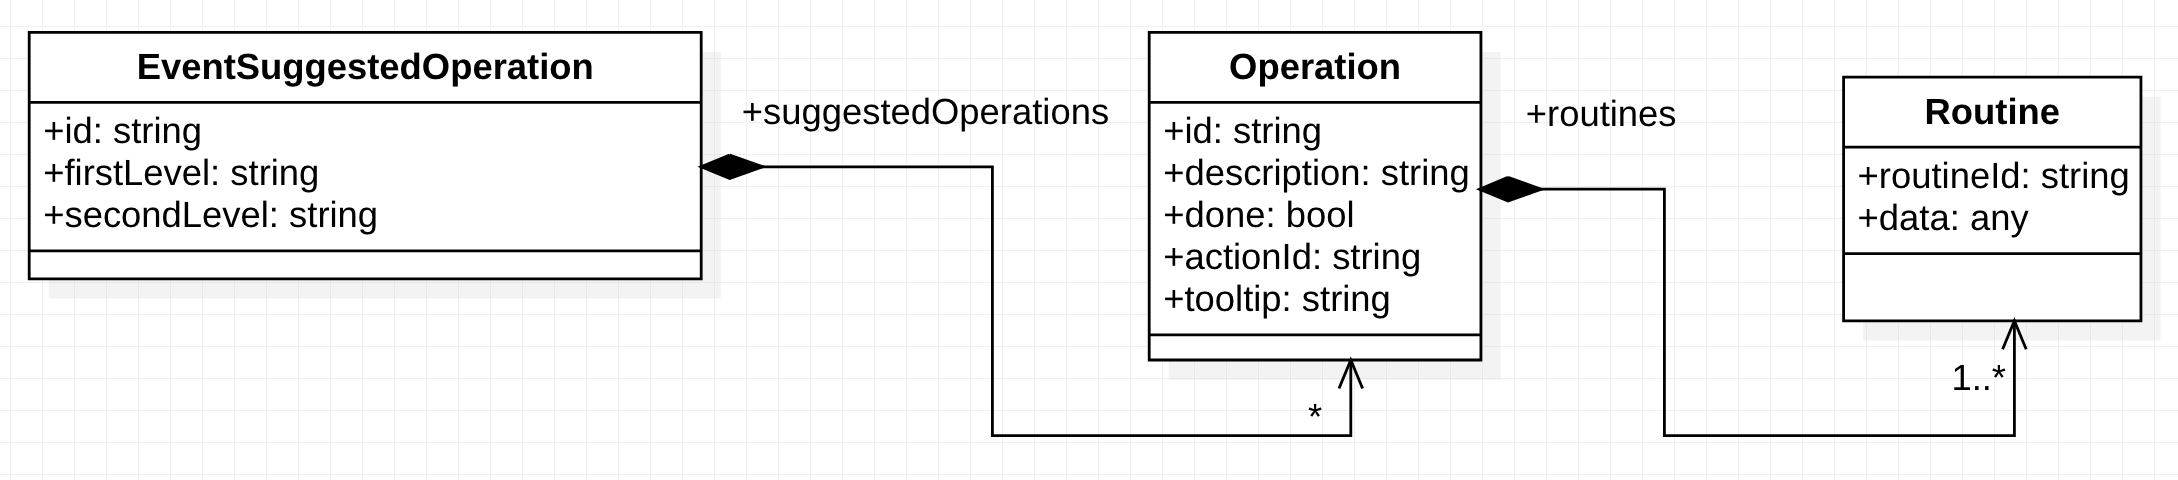
\includegraphics[width=150mm]{img/class_diagram}
    \caption{Class Diagram}
  \end{figure}

Per ogni evento previsto dal sistema è associata l'entità \textbf{EventSuggestedOperation}, che contiene una collezione
di \textbf{Operation}, queste consistono nelle operazioni che dovrà effettuare l'operatore per completare la risposta 
all'evento accaduto. l'attributo \emph{tooltip} conterrà un eventuale suggerimento che verrà visualizzato al passare del 
mouse. \emph{actionId} indica invece il tipo di operazione da effettuare per concludere tale operazione. Il booleano \emph{done} invece indica se suddetta 
operazione è stata effettuata o meno. Ogni operazione ha una collezione di \textbf{routines}, che servono a automatizzare il compimento 
di quest'ultima, facilitando l'esperienza utente. Ogni routine ha una payload contenuto nell'attributo \emph{data}.


\subsection{Scelta del sistema di comunicazione}
Il componente, chiamato \textbf{SuggestedOperationWidget}, ha bisogno di comunicare con la pagina ospitante con queste modalità:
\begin{itemize}
    \item Se l'operatore conclude un operazione, il \textbf{SuggestedOperationWidget} deve saperlo, e lo sfondo dell'operazione 
    appena effettuata deve risultare verde
    \item quando si sceglie di eseguire un operazione dal widget, questo deve inviare alla pagina ospitante le routines collegate
\end{itemize}

Per effettuare queste comunicazioni è stato adottato \textbf{Broadcast Channel API}, il quale è stato già introdotto precendetemente.

Si vanno quindi a definire due canali di comunicazione:
\begin{itemize}
    \item \textbf{po.actions}: per comunicare dalla pagina ospitante al componente le azioni che sono state effettuate dall'operatore.
    \item \textbf{sow.routines}: permette al componente di inviare le routines necessarie al compimento dell'operazione alla pagina ospitante
\end{itemize}
\begin{figure}[H]
    \centering
    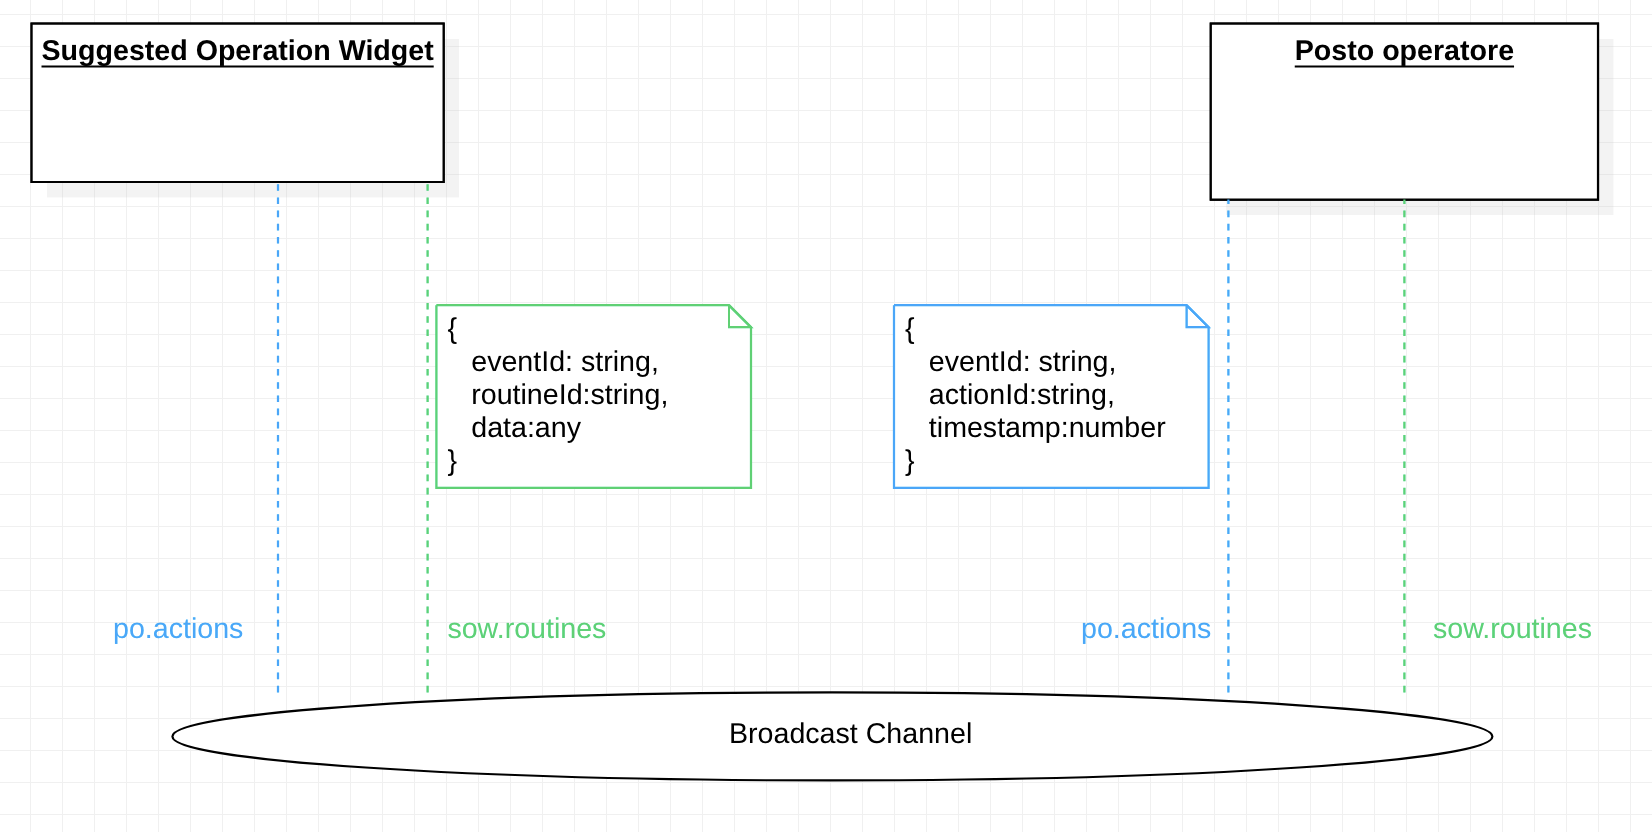
\includegraphics[width=150mm]{img/broadcast_channel}
    \caption{Schema del broadcast channel}
  \end{figure}


\pagebreak
\subsection{Angular}
Si è scelto di creare il componente con Angular, in quanto viene già usato per il resto del progetto di Leonardo.

Angular è un framework di progettazione per applicazioni e una piattaforma di sviluppo per la creazione 
di SPA efficienti e sofisticate. \cite{angular}

Si è creato quindi un Component Angular, il quale consiste in:
\begin{itemize}
    \item Un template HTML che definisce l'aspetto
    \item Una classe Typescript che definisce la logica
    \item Un selettore per definire come il componente è usato nel template
    \item un foglio di stile CSS
\end{itemize}

Creare un fragment microfrontend con Angular è molto semplice, perchè il framework mette a disposizione il concetto di 
\textbf{Angular Elements}, che consiste nell'incapsulare un componente in un Web Component.

Il package \emph{@angular/elements} esporta il metodo \emph{createCustomElement()}, che mette a disposizione un ponte tra
l'interfaccia del componente Angular e le funzionalità di riconoscimento dei cambiamenti presenti nelle API javascript.

L'obiettivo è quello di convertire anche gli altri componenti della applicazione web in Angular Elements, tutti provenienti da app diverse,
sviluppate da team diversi.
Un problema che è stato riscontrato durante il tirocinio è che di base non possono coesistere più app Angular nella solita pagina.
Questo è dovuto ad un limite di compilazione: Angular utilizza Webpack per creare il bundle dell'app, creando un oggetto \textbf{window.webpackJsonp}.
Il nome dell'oggetto non è modificabile, quindi eventuali altre app che si eseguono nella pagina causeranno un conflitto di namespacing, causando
il malfunzionamento dell'app. \cite{webpackModifica}

Per rinominare l'app abbiamo scelto la libreria \textbf{Npx Build Plus}, definendo un semplice comando per chiedere a Webpack di 
dare un nome univoco:

module.exports = {
    output: {
        library: 'suggOpWidget'
    }
};


E' stato realizzato inoltre una repository pubblica su Github, che fungerà da esempio per i prossimi componenti. 
Questa contiene un Angular Element già correttamente configurata e pronta per essere compilata e 
per coesistere con più fragment in un'unica pagina.\cite{repogit}

\section{Sviluppo}
Il codice del componente comprende principalmente i seguenti files:
\begin{itemize}
    \item Le interfacce:
    \subitem eventOperation.model.ts
    \subitem suggestedOperation.model.ts
    \subitem routine.model.ts
\end{itemize}

\begin{itemize}
    \item Il componente:
    \subitem suggested-operation-widget.component.ts
    \subitem suggested-operation-widget.component.html
    \subitem suggested-operation-widget.component.scss
\end{itemize}

\begin{itemize}
    \item I servizi:
    \subitem events.service.ts
 \end{itemize}

 La logica del componente risiede principalmente nel servizio \textbf{events}.
 Per limitare le connessioni al server si effettua una cache delle operazioni suggerite scaricate dal database.
 Quando il componente si avvia, controlla se è presente una cache e se è aggiornata, in caso contrario si effettua una richiesta
 al server.
 La cache trattiene anche gli storici delle operazioni già effettuate, marcate come "done", 
 per mantenerle anche nelle successive sessioni del browser.



\subsection{Sequence diagram}

\begin{figure}[H]
    \centering
    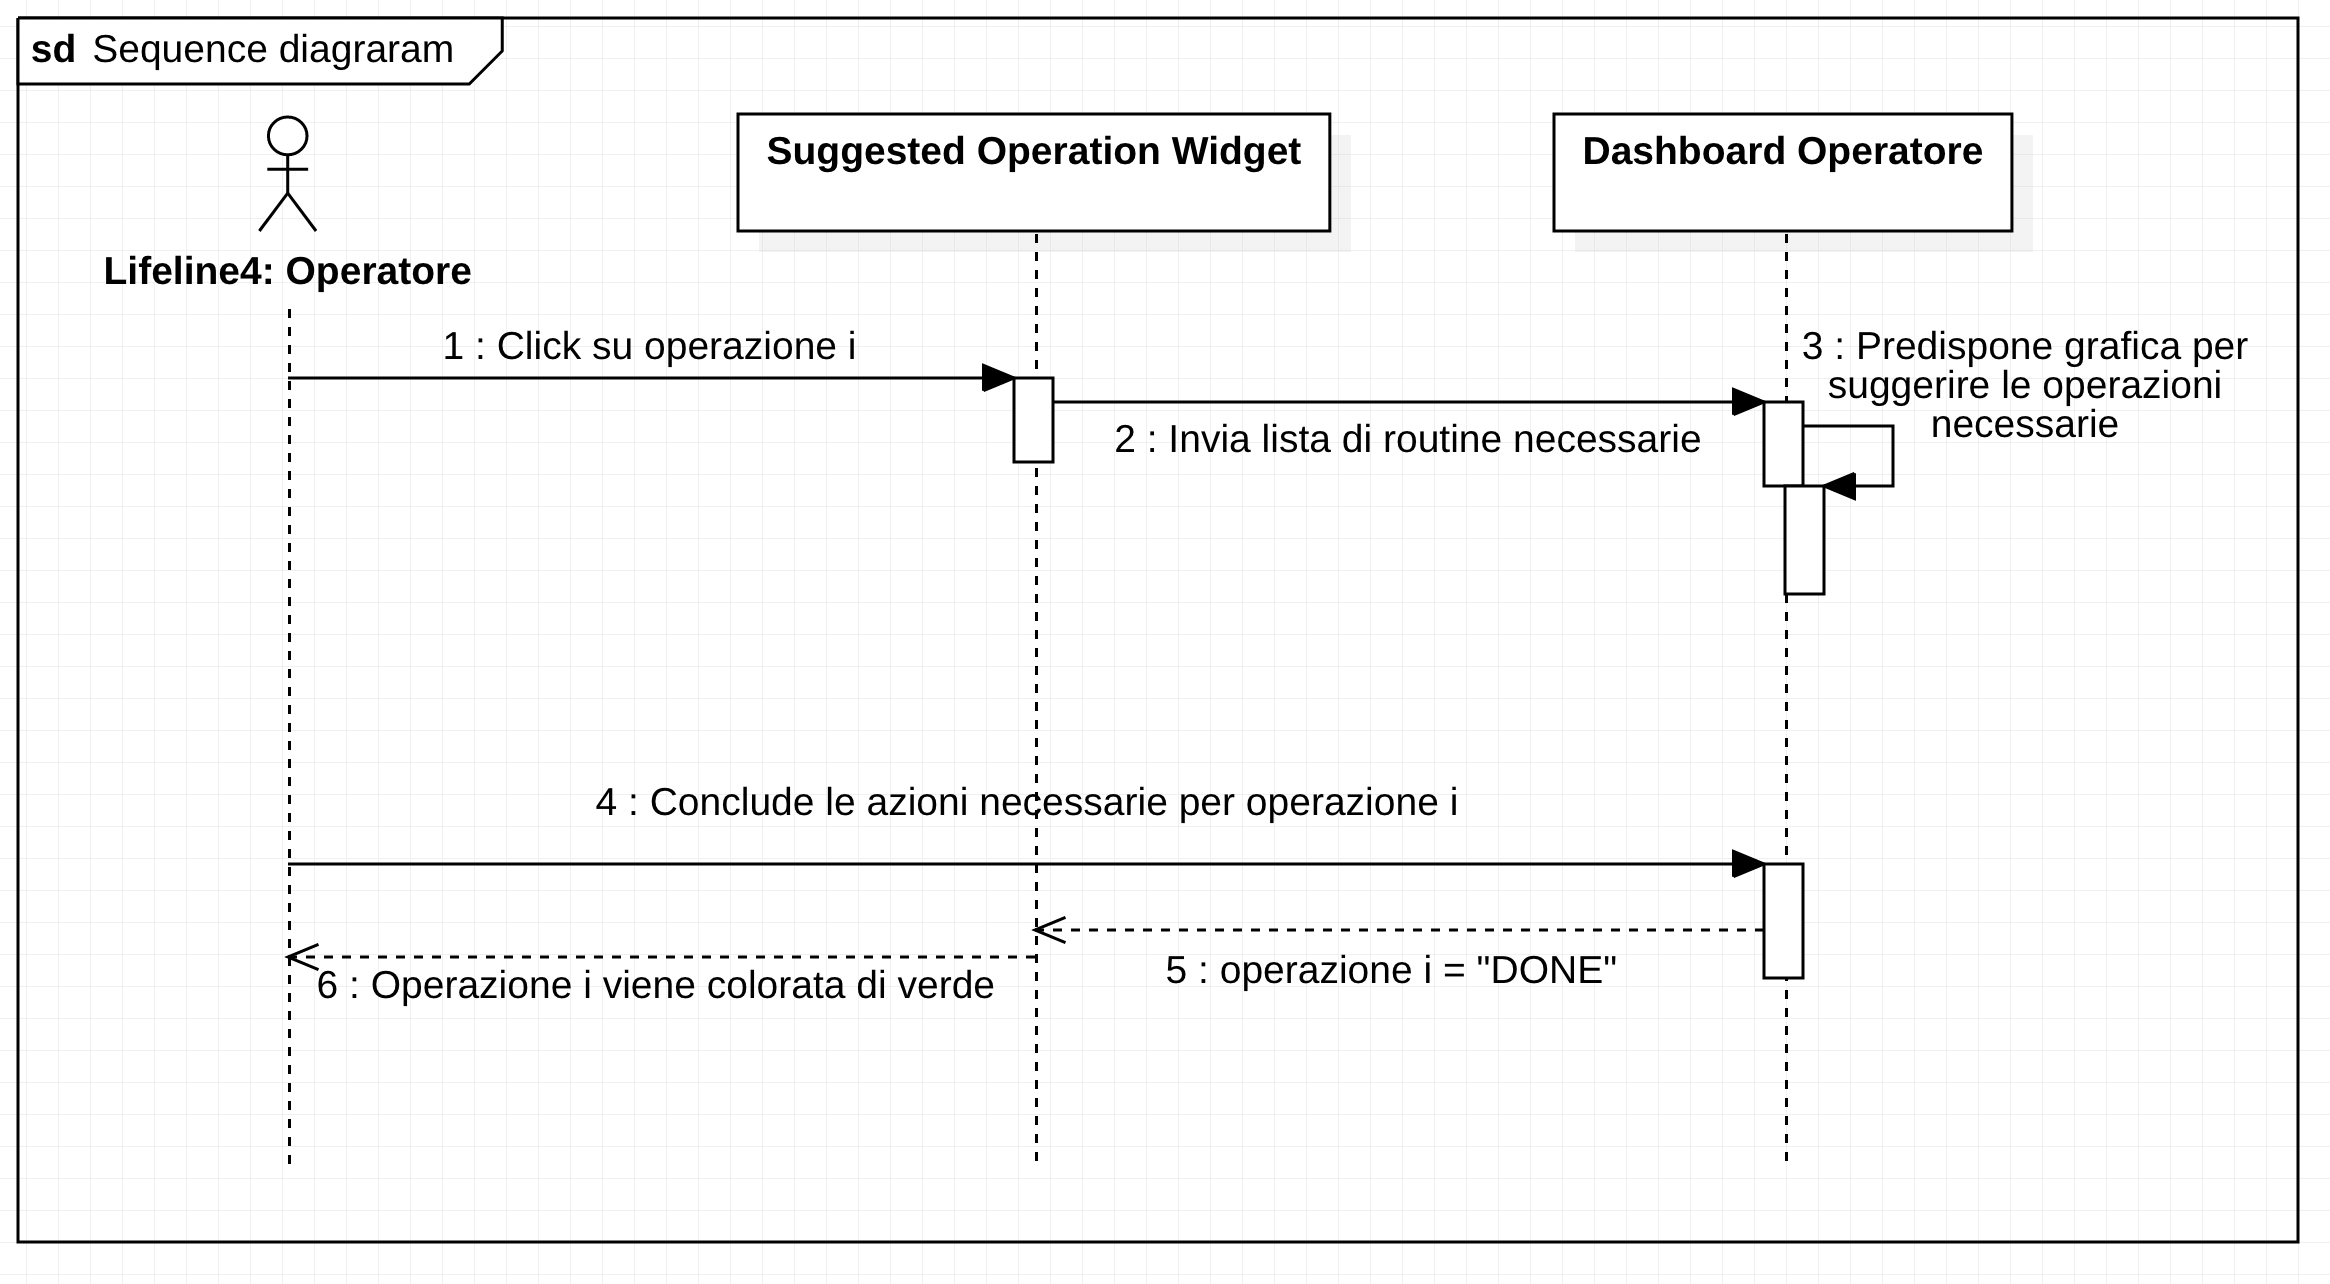
\includegraphics[width=150mm]{img/sequence}
    \caption{Sequence diagram che mostra l'interazione dell'operatore con il componente}
  \end{figure}


\subsection{User Design}

\subsection{Problemi riscontrati}

\pagebreak
\section{Sviluppi futuri}